\clearpage
\section*{Archived supplied-graph formulation and results}
The following original formulation and result sections concern the reduced V35 supplied-graph mechanism. Its public facility coordinates, 18-action common prefix, 1\,m motion, diagnostic recursion and floor-exposure stopping requirement are not the main unknown-exploration policy. All original outcome tables and negative results are retained. Historical figure and table numbers in prose refer to that archived presentation; cross-referenced items are renumbered here.
\hypertarget{problem-formulation}{%
\section{Problem Formulation}\label{problem-formulation}}

Each acquisition task takes place in a static environment; changes occur between tasks. The local inspection target is one equipment-scale facility with an unknown configuration \(h\in\{0,1\}\). Both policies receive two public templates, a facility coordinate frame, an initial pose \(s_0\), and a safe pose graph. They receive RGB-D, planar scan, and pose observations only when those observations are acquired. The category--configuration association is manually specified public knowledge. Evaluation references, true configuration identifiers, and actual measurements from unexecuted actions are unavailable to the planner.

A forward motion of 1 m or a 90\ensuremath{^{\circ}} turn consumes one action and acquires a sensor frame. An identical 18-action observation prefix precedes autonomous selection within total budget \(B\). The original confirmation uses \(B=42\); the extension also evaluates 30 and 54. A qualified task must remain collision-free, finish within budget, attain at least 80\% planar coverage, and return to the initial position and orientation. The experiment consequently tests allocation after common observation, rather than unknown-environment exploration from the first action.

The principal measured score combines planar coverage and surface quality:

\[
C_{\rm map}=\frac{|\{c\in\mathcal R:m_T(c)\ne-1\}|}{|\mathcal R|},
\qquad F_{1,\tau}=\frac{2P_\tau R_\tau}{P_\tau+R_\tau},
\qquad J_5=C_{\rm map}F_{1,0.05}.
\]

Here \(\mathcal R\) is the start-reachable evaluation grid, \(m_T\) is the terminal measured occupancy map, and \(-1\) denotes an unobserved cell. \(P_\tau\) and \(R_\tau\) denote surface precision and recall within distance \(\tau\), measured in meters. Section~\ref{experimental-setup-and-matched-comparisons} specifies the evaluation region, sampling, and qualification rules.

The desired policy maximizes expected measured \(J_5\) using acquired information while respecting budget and return constraints. Online template exposure is only its planning surrogate. A larger predicted opportunity need not produce a more accurate fused mesh, and additional observations do not guarantee improvement at every surface threshold.

\hypertarget{observation-planning-with-correctable-category-priors}{%
\section{Observation Planning with Correctable Category Priors}\label{observation-planning-with-correctable-category-priors}}

\hypertarget{system-overview-and-planning-state}{%
\subsection{System overview and planning state}\label{system-overview-and-planning-state}}

The NSO research prototype selects observation actions using a configuration belief and the budget required to return. Figure 1 separates four functions: category support supplies an initial preference, geometric correction revises it, diagnostic planning evaluates feasible continuations, and a return-feasibility check admits the next action (Table 1). Each executed action acquires a new measurement for replanning and measured reconstruction. The category-conditioned policy S and geometric control G share the graph, public templates, diagnostic planning, and fusion backend; only S receives the category prior. The shared controls limit attribution of individual mechanisms.

\begin{table}[!htbp]
\caption{Functional components and their roles in the observation loop}\label{tab:1}
\small\renewcommand{\arraystretch}{1.12}\setlength{\tabcolsep}{3pt}
\setlength{\JournalTableWidth}{\dimexpr\linewidth-4\tabcolsep\relax}
\begin{tabular}{@{}>{\raggedright\arraybackslash}p{0.16\JournalTableWidth} >{\raggedright\arraybackslash}p{0.32\JournalTableWidth} >{\raggedright\arraybackslash}p{0.52\JournalTableWidth}@{}}
\toprule
Function & Input & Output and role \\
\midrule
Category support & Acquired RGB, pose, measured-map summary & Register category support and configuration prior \\
Diagnostic planning & Graph, exposure sets, beliefs, remaining budget & Compare feasible continuations and select a subgoal \\
Return-feasibility check & Proposed edge, budget, return distance & Permit or reject the executable action \\
Geometric correction & Acquired depth/scan and public predictions & Bound geometric evidence and revise belief \\
\bottomrule
\end{tabular}
\end{table}

\begin{figure}[!htbp]
\centering
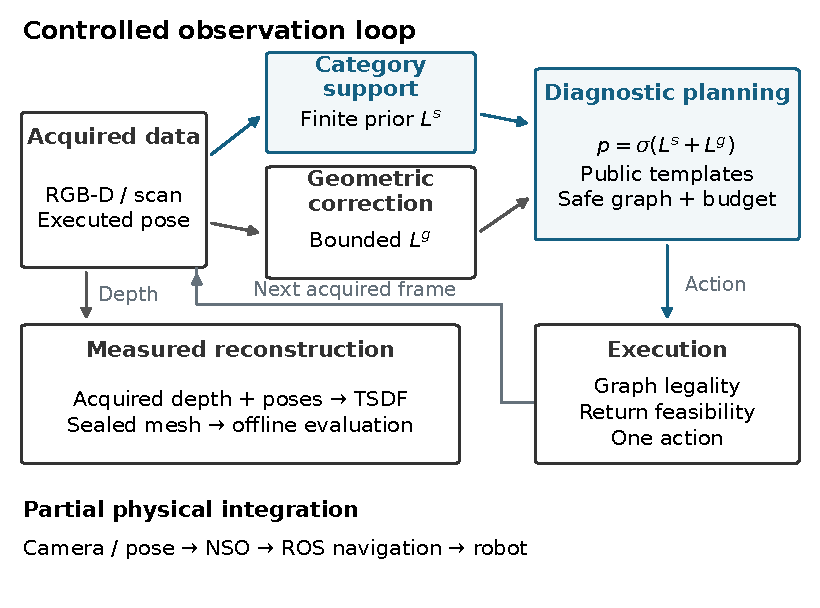
\includegraphics[width=\linewidth,height=.67\textheight,keepaspectratio]{Fig1.pdf}
\caption{Information flow and execution boundary. Category support and acquired geometric evidence update a configuration belief; the planner selects a feasible observation action. Acquired depth separately updates the measured reconstruction. Public predictions score candidate actions and never become fused measurements. The robot interface is an integration path whose current evidence is reported separately in Section~\ref{physical-deployment}}\label{fig:1}
\end{figure}

After action \(t\), the planning state is

\[
x_t=(s_t,b_t,M_{0,t},M_{1,t},p_t,\mathcal V_t),\qquad b_t=B-t.
\]

Here \(s_t\) includes position and heading, \(p_t\) weights configuration 0, and \(\mathcal V_t\) contains measured poses. Each \(M_{h,t}\) records the union of floor samples and surface patches predicted visible from previously observed poses under public template \(h\). These exposure sets support prospective planning; the measured map separately integrates acquired depth. Neither hidden configuration identifiers nor evaluation surfaces enter the state. The common 18-action prefix updates observations and returns to \(s_0\); subsequent actions depend on the resulting belief.

Both hypotheses remain available throughout execution. Category information changes their weights rather than selecting a template as reconstructed truth. The online belief module additionally retains geometric log-support and category-registration history, while each planning call receives their current combined weight. This separates two questions: which configuration the acquired evidence supports, and which affordable observation sequence is valuable under that uncertainty.

\hypertarget{category-support-and-geometric-correction}{%
\subsection{Category support and geometric correction}\label{category-support-and-geometric-correction}}

A category cue must influence early decisions without preventing later contradictory measurements from changing the route. We therefore register finite category support once and combine it with bounded evidence from newly acquired viewpoints. This design allows a cue to establish a preference while preserving both configuration hypotheses.

The category-support function registers a category when its marker occupies at least 16 exact-color pixels at each of two distinct XY positions, without a competing marker in those frames. Registration supplies \(L_t^s=\pm\log9\); repeated detections do not multiply this prior, and conflicting category support clears it. G uses \(L_t^s=0\). Synthetic markers provide a controlled category channel, independently of natural-image recognition performance.

Geometric correction compares acquired depth and scan measurements with both public predictions. Let \(e_{h,t}^{k}\) be the mean residual loss for eligible modality \(k\) under template \(h\), and \(\mathcal K_t\) its valid-modality set. At a newly visited pose,

\[
\begin{aligned}
\delta_t=\operatorname{clip}_{[-6,6]}
\left(\frac{1}{|\mathcal K_t|}\sum_{k\in\mathcal K_t}
\bigl(e_{1,t}^{k}-e_{0,t}^{k}\bigr)\right),\\
L_t^g=\operatorname{clip}_{[-24,24]}(L_{t-1}^g+\delta_t),\qquad
p_t=\sigma(L_t^g+L_t^s).
\end{aligned}
\]

Here \(\sigma(z)=(1+e^{-z})^{-1}\). The increment is zero when no modality qualifies or the pose has already supplied evidence. Residuals use samples where public predictions differ by more than \(10^{-5}\) m. Depth requires eight valid pixels and normalized disparity residual \((57.6/z-57.6/\widehat z_h)/0.25\); scan requires three valid beams and residual \((r-\widehat r_h)/0.02\). Each sample contributes half its squared residual, capped at 12.5. Missing measured returns are ignored; a missing predicted depth return receives the capped loss. Eligible modality means receive equal weight.

These bounded pseudo-likelihoods prevent individual extreme residuals from dominating. They are not calibrated probabilities, and excluding exact repeats does not establish independence between neighboring views. New depth from a repeated pose still contributes to fusion. An incorrect prior remains correctable: for \(L^s>0\), configuration-1 support reaches \(\eta>1/2\) whenever

\[
L_t^g\le-L^s-\operatorname{logit}(\eta).
\]

This threshold is attainable only if sufficient contrary observations occur and the cumulative cap permits it. The finite prior therefore expresses a revisable preference rather than a permanent semantic constraint.

\hypertarget{predictive-value-and-diagnostic-lookahead}{%
\subsection{Predictive value and diagnostic lookahead}\label{predictive-value-and-diagnostic-lookahead}}

A diagnostic view can be valuable because it changes a later route choice, even when its immediate predicted surface gain is small. The planner therefore evaluates future exposure under both configurations and includes one possible diagnostic event within each planning call. Its predicted exposure score guides sensing, while the endpoint score remains a measurement of the reconstructed surface.

For template \(h\), let \(\mathcal F_h\) contain its floor samples, \(\mathcal P_h\) its exterior vertical patches, \(a_u\) the patch area, and \(A_h\) the total exterior vertical area. Writing \(M_h^f\) and \(M_h^s\) for the corresponding exposed subsets gives

\[
\widetilde C_h=\frac{|M_h^f|}{|\mathcal F_h|},\qquad
\widetilde S_h=\min\left(1,\frac{\sum_{u\in M_h^s}a_u}{A_h}\right),\qquad
\widetilde J_h=\widetilde C_h\widetilde S_h.
\]

Thus \(\widetilde S_h\) is an exposed-area fraction, not reconstructed surface F1. The surrogate rewards opportunities to observe missing surfaces but does not model TSDF error or improvements from repeated measurements. Its relation to measured \(J_5\) is tested empirically.

Exposure is accumulated by set union, so viewing an already exposed patch supplies no additional proxy area. Changing direction can still reveal previously occluded patches. Floor samples are those declared by the public planning model, distinct from the finer reachable-cell grid used to measure \(C_{\rm map}\). Consequently, neither component of the surrogate is substituted for an endpoint measurement. Keeping both representations makes the planning assumption explicit: access to additional surface area is a useful, imperfect predictor of reconstructed quality.

Let \(M=(M_0,M_1)\). Stopping requires the complete initial pose and adequate predicted floor exposure under both configurations:

\[
Z(s,M,p)=
\begin{cases}
p\widetilde J_0(M_0)+(1-p)\widetilde J_1(M_1),
&s=s_0,\ \min_h\widetilde C_h(M_h)\ge0.8,\\
-\infty,&\text{otherwise}.
\end{cases}
\]

Diagnostic planning approximates belief-space planning \cite{ref12,ref13} with one future diagnostic event per planning call. Diagnostic candidates are determined from public sensor predictions: treating each template prediction as a hypothetical observation must yield geometric evidence at least \(+\log99\) for configuration 0 and at most \(-\log99\) for configuration 1. Previously measured poses are excluded. This identifies potentially discriminative viewpoints without obtaining their actual observations.

For an anticipated diagnosis of assumed accuracy \(r_d=0.99\), the branch weights and updated planning beliefs are

\[
\begin{aligned}
\lambda_0&=pr_d+(1-p)(1-r_d),\qquad \lambda_1=1-\lambda_0,\\
p^{(0)}&=\frac{pr_d}{\lambda_0},\qquad
p^{(1)}=\frac{p(1-r_d)}{\lambda_1}.
\end{aligned}
\]

Let \(q\in\{0,1\}\) indicate whether this event remains available. Action \(a\) reaches \(s'\), consumes one action, and updates \(M'_h=M_h\cup E_h(s')\), where \(E_h\) is public predicted exposure. The continuation and value recursions are

\[
Q_q(a)=
\begin{cases}
\sum_{y=0}^{1}\lambda_y V_0(s',b-1,M',p^{(y)}),
&q=1,\ s'\text{ diagnostic},\\
V_q(s',b-1,M',p),&\text{otherwise},
\end{cases}
\] \[
V_q(s,b,M,p)=\max\left\{Z(s,M,p),\max_{a\in\mathcal A(s)}Q_q(a)\right\}.
\]

At \(b=0\), only stopping is available. States whose return distance exceeds \(b\) are infeasible, as are diagnostic actions with either infeasible branch. Forecast beliefs remain inside the current calculation. The controller executes only the first selected action, updates belief from acquired measurements, and replans. The category strength 0.9 and forecast accuracy 0.99 are fixed design settings shared across the comparisons, rather than measured classifier or sensor accuracies.

The recursion evaluates complete remaining continuations, rather than immediately visible area alone. Anticipated diagnosis is useful only through the different actions it may enable afterward. Requiring a feasible continuation in both branches prevents a low-weight configuration from being silently discarded to satisfy the return and coverage gates. The approximation limits the number of belief changes within one forecast; it does not limit the number of measured corrections over the executed trajectory. A later call can anticipate another diagnostic event after assimilating the latest frame.

\hypertarget{budgeted-execution-and-reconstruction}{%
\subsection{Budgeted execution and reconstruction}\label{budgeted-execution-and-reconstruction}}

An informative view is useful only if the robot can execute it and still return within budget. The execution layer reserves the shortest graph return cost before each action; the reconstruction layer then integrates only the depth acquired at the executed pose.

The return-feasibility check accepts a legal edge only if

\[
1+d_{\rm return}(s')\le b_t,
\]

where return distance includes restoration of the starting heading. On the fixed graph with unit action costs, this preserves an affordable return path: after each accepted action, \(d_{\rm return}(s_{t+1})\le b_t-1=b_{t+1}\). This certificate concerns graph feasibility; task qualification additionally requires measured coverage, collision-free execution, and actual return.

\par\medskip\noindent\begin{minipage}{\linewidth}
\small\hrule\vspace{0.6em}
\textbf{Algorithm 1. Category-conditioned receding-horizon observation.}

\begin{verbatim}
Input: common graph, templates, budget B, prefix, policy G or S
Initialize belief support, exposures, and visited poses
Repeat:
  Read the initial frame or latest executed-action frame
  Fuse acquired depth exactly once into the measured TSDF
  Register category support and update geometric evidence
  Add current template exposures and record the measured pose
  If collision or budget exhaustion: record termination; exit
  If the shared prefix is unfinished: select its next action
  Otherwise:
    Exclude measured poses from diagnostic candidates
    Solve V1 from the current state and remaining budget
    If infeasible or a resource cap is exceeded: fail; exit
    If stopping is optimal within tolerance: stop; exit
    Select the first maximizing action in fixed graph-edge order
  Check graph legality and the return-budget inequality
  If rejected: record the termination reason; exit
  Execute one action, charge its cost, and obtain the next frame
Output: measured map, trajectory, observations, and stop reason
\end{verbatim}
\vspace{0.4em}\hrule
\end{minipage}\par\medskip


Equal-valued choices use a \(10^{-12}\) tolerance and fixed edge order. The shared Open3D CPU TSDF \cite{ref4,ref11} uses 4 cm voxels and 12 cm truncation; public templates never contribute synthetic depth. Outputs precede independent endpoint evaluation. Incorrect-prior controls exchange category interpretation; the no-correction variant additionally disables measured correction and forecast diagnosis.

For \(N\) poses and exposure bitset lengths \(m_0,m_1\), the cached state count is conservatively bounded by \(K\le3N(B+1)2^{m_0+m_1}\), covering the initial and two post-diagnosis weights. With maximum out-degree \(d\), bitset-update cost \(T_m\), and terminal-evaluation cost \(T_z\), planning costs \(O(K(dT_m+T_z))\), excluding return-distance preprocessing. Each call permits 1.5 million cached states and approximately 20 s; elapsed time is checked every 1024 new states and at selection completion. This finite implementation supports the controlled task, with exponential exposure-state dependence.

\hypertarget{decision-interpretation-and-conditions-for-benefit}{%
\subsection{Decision interpretation and conditions for benefit}\label{decision-interpretation-and-conditions-for-benefit}}

A recorded example connects the recursion to robot behavior. After the common prefix in P00, G assigns both configurations weight 0.5; left/right continuation values of 0.650944 tie. With configuration-1 category support 0.9, S obtains 0.668008/0.711865 and turns right at action 19. A misleading prior can subsequently reverse: geometric evidence of \(-6\) at step 28 gives configuration-1 weight \(1-\sigma(-6+\log9)=0.978178\), followed by a changed action at step 29. These are planning values and belief weights; measured reconstruction outcomes are reported separately.

The underlying tradeoff can be expressed using established belief-based decision principles \cite{ref12,ref13}. Assume two initially equally likely configurations, two return-feasible routes, matched utility \(U_+\), mismatched utility \(U_-\), and \(\Delta=U_+-U_->0\). A category cue has symmetric reliability \(r_c\ge1/2\). Optional geometric diagnosis has symmetric reliability \(r_d\ge1/2\), is conditionally independent given configuration, and costs utility \(\kappa\). Both routes remain feasible afterward. For current belief \(p\), direct choice succeeds with probability \(m=\max(p,1-p)\); optimal choice after diagnosis succeeds with probability \(\max(m,r_d)\). Its net value is

\[
\Delta\max(0,r_d-m)-\kappa.
\]

G benefits from diagnosis when \(\kappa<(r_d-1/2)\Delta\), whereas a category-conditioned decision requires \(\kappa<(r_d-r_c)_+\Delta\), with \(\kappa\ge0\). An informative cue can therefore avoid a diagnostic detour while preserving a useful observation direction. Its benefit disappears when geometry already resolves the choice or route utilities coincide. When \(r_d\ge r_c\) and diagnosis is free, both policies can attain the same expected directional utility; a free but less reliable diagnosis need not remove the category advantage. These analytical reliabilities are assumptions distinct from implementation settings. The argument identifies conditions for improved allocation; it does not guarantee better measured reconstruction under the exposure surrogate.

The practical consequence is a conditional experimental prediction: a category cue should matter when it changes a consequential route ranking before equivalent geometric evidence is affordable. If geometry and category already favor the same route, identical actions and quality are expected. Tests therefore examine action changes, acquired surfaces, and measured quality together, rather than interpreting stronger belief alone as a mapping improvement.

\hypertarget{experiments-and-results}{%
\section{Experiments and Results}\label{experiments-and-results}}

The controlled experiments test category-conditioned observation at matched coverage, geometric correction, and sensitivity to budget and changed backgrounds. Sections~\ref{joint-exploration} and~\ref{physical-deployment} evaluate unknown-exploration and physical deployment separately.

\hypertarget{experimental-setup-and-matched-comparisons}{%
\subsection{Experimental setup and matched comparisons}\label{experimental-setup-and-matched-comparisons}}

The simulator supplies 96\ensuremath{\times}72 depth images over a 4 m range and a 360\ensuremath{^{\circ}} planar scan with 180 beams over 8 m. Poses are exact. Depth noise has a standard deviation of 0.25 pixels in reference disparity; no additional random scan noise is applied. The experiments isolate planning under controlled observations rather than reproduce physical sensor errors.

The evaluator derives the start-reachable safe-cell set \(\mathcal R\) using a 0.2 m grid and 0.2 m robot radius. It contains 588 cells in P00 and 668 in P01. A nonunknown cell counts as observed, including one marked occupied, so coverage is not occupancy-classification accuracy. Ground truth is used after prediction sealing, not to supply runtime measurements.

Surface precision and recall follow distance-threshold comparison \cite{ref14}. Precision queries the reference from sampled predicted surfaces; recall queries the prediction from fixed exterior vertical reference surfaces. The prediction is cropped to the common bounding box of both templates with a 0.20 m margin, and the known ground is removed. Thus, errors outside this region do not enter precision. No registration or hole filling is applied. Thresholds are fixed at 2, 5, and 10 cm, with 5 cm primary; empty predictions receive zero quality. Coverage, precision, recall, and task qualification accompany the product to avoid hiding its components.

Confirmation freezes the controller and uses a held-out noise seed on two previously seen parent layouts, each with two configurations: eight runs and four G/S pairs. The layout-level units are the two parent layouts. Two configurations per layout and repeated noise realizations are paired conditions, not independent evidence of category-level generalization. The policies differ as follows: G has no category support; S uses the designated correct cue; X reverses the category interpretation; and Xnf uses the same reversed interpretation while disabling measured correction and future diagnostic anticipation. The historical development X/Xnf contrast therefore evaluates the bundled correction policy; the separate factorial below isolates its two switches. Replays and alternative thresholds reuse these trajectories; they do not increase the number of independent layouts or trials. The principal G control retains the diagnostic views and revisiting available to S; Xnf deliberately disables measured correction and anticipated diagnosis.

For each matched condition we report the absolute score difference, \(\Delta J_5=J_{5,S}-J_{5,G}\). A relative mean change is \(100(\overline J_{5,S}/\overline J_{5,G}-1)\), rather than an average of per-condition percentages. Qualification is reported over all declared attempts; endpoint means include only the explicitly qualified groups.

The recorded software is Python 3.12.3, NumPy 1.26.4, SciPy 1.11.4, and Open3D 0.19.0, with one OpenMP, OpenBLAS, and MKL thread. No GPU is required. Figures use actual recorded actions and measured meshes except the explicitly schematic architecture diagram.



\hypertarget{surface-reconstruction-at-matched-coverage}{%
\subsection{Surface reconstruction at matched coverage}\label{surface-reconstruction-at-matched-coverage}}

Across the four confirmation conditions in Table 2, mean \(J_5\) increases from 0.702576 to 0.745881, a relative improvement of 6.1638\%. Every run uses 42 actions, avoids collision, and returns exactly. Mean coverage is identical at 0.952544; mean surface F1 increases from 0.737490 to 0.782951. This decomposition attributes the observed joint-score gain to surface reconstruction at matched planar coverage.

\begin{table}[!htbp]
\caption{Complete confirmation pairs; relative change compares policy means}\label{tab:2}
\small\renewcommand{\arraystretch}{1.12}\setlength{\tabcolsep}{3pt}
\setlength{\JournalTableWidth}{\dimexpr\linewidth-6\tabcolsep\relax}
\begin{tabular}{@{}>{\raggedright\arraybackslash}p{0.32\JournalTableWidth} >{\raggedright\arraybackslash}p{0.22\JournalTableWidth} >{\raggedright\arraybackslash}p{0.22\JournalTableWidth} >{\raggedright\arraybackslash}p{0.24\JournalTableWidth}@{}}
\toprule
Layout/configuration & G: \(J_5\) & S: \(J_5\) & S\ensuremath{-}G \\
\midrule
P00/h0 & 0.772200 & 0.772200 & 0 \\
P00/h1 & 0.672703 & 0.760456 & +0.087753 \\
P01/h0 & 0.727281 & 0.727281 & 0 \\
P01/h1 & 0.638118 & 0.723586 & +0.085468 \\
Mean & 0.702576 & 0.745881 & +0.043305 \\
\bottomrule
\end{tabular}
\end{table}

In both h1 cases, category conditioning changes the first autonomous turn. The resulting surface recall rises from 0.5958 to 0.7249 in P00 and from 0.5555 to 0.6845 in P01. Both h0 pairs follow identical trajectories. The relative mean gains at 2 and 10 cm are 5.5040\% and 6.2110\%, respectively. These descriptive sensitivities do not establish statistical significance across unseen layouts. The primary outcome pattern is two wins, two ties, and no losses across four configuration pairs; the two ties are exact trajectory and metric matches. We therefore report every pair and the absolute mean difference of 0.043305 alongside the relative mean change. No confidence interval treating configurations, seeds, frames, or checkpoints as independent layouts is used.



Retained endpoint meshes show the recovered side structures using matched cameras and scales. P00/h1 needs 28 m and 14 turns for G versus 26 m and 16 turns for S; P01/h1 uses 28 m and 14 turns for both. Every run acquires the same number of frames. The effect therefore depends on allocating observations differently, rather than increasing sensing or travel.



\hypertarget{geometric-correction-and-reconstruction-progress}{%
\subsection{Geometric correction and reconstruction progress}\label{geometric-correction-and-reconstruction-progress}}

The P00 development timeline connects the decision example in Section 4.5 to acquired evidence. Category support changes the first autonomous observation direction at action 19, while subsequent geometric measurements can reverse the influence of an incorrect cue.

With the incorrect cue, X initially assigns configuration 1 a weight of 0.1. At step 28, 1092 informative depth pixels provide sufficient contrary evidence to raise this weight to 0.978178. X then moves forward at action 29, while Xnf turns right. Across the two development configurations, X improves mean \(J_5\) over Xnf from 0.655065 to 0.672254, or 2.6241\%. Because Xnf also removes anticipated diagnosis, this is not an isolated posterior-update ablation. At the stricter 2 cm threshold, the h1 difference is \ensuremath{-}0.00216, indicating that correction does not improve every surface-scale measure.




\paragraph{Measured Correction and Forecast Diagnosis.}
A separately frozen $2\times2$ factorial separates measured posterior correction from forecast diagnostic anticipation (Table~\ref{tab:archived-correction-factorial}). All eight routes use the same regenerated public cache for P00, its two configurations, the fixed incorrect category interpretation, a 42-action budget, an 18-action common prefix, and disparity-noise seed 1901. The original renderer, planner, return rules, fusion backend and evaluator are retained. Four endpoint equivalence runs compare the wrapper with the original X and Xnf controllers on identical acquired packets; every action, posterior and planning receipt agrees. These implementation checks are excluded from the eight factorial routes. The eight routes represent one parent layout and two related configurations, with no additional independent layout replication; their endpoints are not pooled with the older development-cache results.

\begin{table}[!htbp]
\caption{Complete correction factorial on one P00 parent and two configurations: eight actual simulated routes with a common public cache, wrong prior, budget 42, prefix 18 and noise seed 1901. All routes return without collision and share $C_{\rm map}=0.957483$. Higher $J_5$ and F1 are better.}
\label{tab:archived-correction-factorial}
\centering\small\renewcommand{\arraystretch}{1.12}
\begin{tabular}{@{}lllrr@{}}
\toprule
Configuration & Measured correction & Forecast diagnosis & $J_5$ & F1 at 5 cm \\
\midrule
h0 & Off & Off & 0.651868 & 0.680814 \\
h0 & Off & On & 0.651868 & 0.680814 \\
h0 & On & Off & 0.669091 & 0.698802 \\
h0 & On & On & 0.669091 & 0.698802 \\
h1 & Off & Off & 0.657205 & 0.686388 \\
h1 & Off & On & 0.657205 & 0.686388 \\
h1 & On & Off & 0.674799 & 0.704764 \\
h1 & On & On & 0.674799 & 0.704764 \\
\bottomrule
\end{tabular}
\end{table}

Measured correction raises mean $J_5$ from 0.654537 to 0.671945, a relative increase of 2.6597\%, within this controlled P00 setting. Forecast diagnosis changes neither trajectory nor endpoint in any of the four matched on/off contrasts: each pair has an identical complete trajectory SHA-256 digest. Thus, the factorial supports a measured-correction effect under these conditions and supplies no observed independent benefit of diagnostic anticipation. It does not show that diagnostic lookahead is generally ineffective, or that the measured-correction gain transfers to other layouts. No confidence interval or significance test treats the eight routes as independent scenes.


We further reintegrate the eight saved confirmation trajectories at 18, 24, 30, 36, and 42 paid actions: 40 measured checkpoints, with unchanged observations, poses, fusion settings, and evaluator. All 16 previously available prefix/endpoint checkpoints reproduce their original metrics exactly. Coverage matches within every pair at every checkpoint and reaches its endpoint value by action 30. Later differences mainly accompany increased surface recall and F1. P00/h1 is still slightly worse for S at action 24 (\ensuremath{-}0.000819), then positive at 30, 36, and 42; P01/h1 is already positive at 24. Both h0 pairs remain tied. Intermediate states may not satisfy return or coverage requirements and are not successful terminal trials.



\hypertarget{sensitivity-to-budget-noise-and-facility-geometry}{%
\subsection{Sensitivity to budget, noise, and facility geometry}\label{sensitivity-to-budget-noise-and-facility-geometry}}

The fixed extension declares 128 trials. Original P00/P01, two configurations, budgets 30/42/54, two noise seeds, and four policies define 96 trials. Two same-family variants at budget 42 add 32: one P00 rib shifts 0.25 m, while three P01 ribs lower their upper boundary from 1.80 to 1.35 m. Transformations apply consistently to both public hypotheses, sensed geometry, and reference surfaces. The safe graph, prefix, controller, and prior settings remain unchanged. These variants test nearby geometry, not unseen natural equipment categories.

All 128 tasks are attempted once: 96 qualify and 32 fail at budget 30 after the common prefix. The controller cannot find a return plan meeting its predicted 80\% coverage gate under both templates. This is a planning-constraint boundary, not universal physical impossibility. Failure maps remain separate from successful endpoint means.

\begin{table}[!htbp]
\caption{Complete extension groups. Each row declares 32 trials; qualified rows contain eight per policy}\label{tab:4}
\small\renewcommand{\arraystretch}{1.12}\setlength{\tabcolsep}{3pt}
\setlength{\JournalTableWidth}{\dimexpr\linewidth-10\tabcolsep\relax}
\begin{tabular}{@{}>{\raggedright\arraybackslash}p{0.26\JournalTableWidth} >{\raggedright\arraybackslash}p{0.148\JournalTableWidth} >{\raggedright\arraybackslash}p{0.148\JournalTableWidth} >{\raggedright\arraybackslash}p{0.148\JournalTableWidth} >{\raggedright\arraybackslash}p{0.148\JournalTableWidth} >{\raggedright\arraybackslash}p{0.148\JournalTableWidth}@{}}
\toprule
Condition/budget & Qualified & G: \(J_5\) & S: \(J_5\) & S/G change & S/G win / tie / loss \\
\midrule
Original/30 & 0/32 & --- & --- & --- & --- \\
Original/42 & 32/32 & 0.702648 & 0.746567 & +6.2505\% & 4 / 4 / 0 \\
Original/54 & 32/32 & 0.926298 & 0.919819 & \ensuremath{-}0.6995\% & 0 / 4 / 4 \\
Variants/42 & 32/32 & 0.704562 & 0.734357 & +4.2289\% & 4 / 4 / 0 \\
\bottomrule
\end{tabular}
\end{table}

The three qualified groups each contain eight G/S pairs, including two noise seeds per geometry/configuration condition. The bundled X/Xnf correction contrast improves its group mean by 1.7328\%, 2.5163\%, and 1.7016\% for original/42, original/54, and variants/42, respectively. These are correction-policy contrasts, not isolated module estimates.

At budget 42, improvements occur in the h1 configurations of both the original and variant layouts, while the h0 routes remain unchanged. At budget 54, the mean difference reverses to \ensuremath{-}0.6995\%, with lower scores in four conditions and unchanged scores in the other four. Coverage reaches 1.0 for both policies; G/S recall is 0.985764/0.983826 and precision 0.873764/0.863789. The negative difference mainly accompanies lower precision, exposing a gap between template exposure and measured reconstruction. This decomposition does not independently identify a fusion-error cause. X also exceeds G/S at this budget, so a correct prior does not guarantee the best measured endpoint under the finite-lookahead surrogate.

The two variants individually improve S/G by 5.0337\% and 3.3974\%. At 2/5/10 cm, original-layout improvements at budget 42 are 5.4991\%/6.2505\%/6.3063\%, whereas budget-54 differences are \ensuremath{-}1.2217\%/\ensuremath{-}0.6995\%/\ensuremath{-}0.2866\%. The reversal is therefore not created by selecting the primary threshold. Noise repeats describe the same geometry and are not additional independent layouts.



\hypertarget{transfer-to-changed-background-layouts}{%
\subsection{Transfer to changed background layouts}\label{transfer-to-changed-background-layouts}}

A background-layout protocol fixes two additional layouts before observing results: a side column removes one right-aisle navigation center, while a rear partition interrupts direct rear passage. Both retain the P00 facility family and public templates. The controller, category mapping, sensor noise rule, fusion, evaluation region, 18-action common prefix, and 42-action budget remain unchanged. All legal safe-grid centers are retained; each new layout has 23 centers and 92 oriented poses. The noise seed is the original confirmation seed, so this test adds two background-layout units, not new noise replicates or unseen facility categories. Each layout uses both configurations and G/S, giving eight tasks and four pairs.

All eight tasks complete 42 paid actions and 43 acquired frames, avoid collision, and return to the full initial pose. Table \ref{tab:5} reports every paired endpoint. Mean coverage is identical at 0.934732; mean precision increases from 0.864441 to 0.870224, recall from 0.672455 to 0.704742, and surface F1 from 0.754450 to 0.777445. Mean joint quality increases from 0.705188 to 0.726215, or 2.9818\%. The gain is concentrated in the rear-partition h1 condition; the other three conditions retain the same trajectories and endpoint quality. Relative differences at 2 and 10 cm are 2.8176\% and 3.1200\%. These are descriptive paired results from two new layouts; configurations do not increase the number of independent layout units.

\begin{table}[!htbp]
\caption{Changed-background results at 5 cm for all four paired conditions. Coverage is equal within each pair; all eight tasks qualify}\label{tab:5}
\small\renewcommand{\arraystretch}{1.12}\setlength{\tabcolsep}{3pt}
\setlength{\JournalTableWidth}{\dimexpr\linewidth-10\tabcolsep\relax}
\begin{tabular}{@{}>{\raggedright\arraybackslash}p{0.26\JournalTableWidth} >{\raggedright\arraybackslash}p{0.148\JournalTableWidth} >{\raggedright\arraybackslash}p{0.148\JournalTableWidth} >{\raggedright\arraybackslash}p{0.148\JournalTableWidth} >{\raggedright\arraybackslash}p{0.148\JournalTableWidth} >{\raggedright\arraybackslash}p{0.148\JournalTableWidth}@{}}
\toprule
Layout / config. & Coverage & G F1 & S F1 & G joint & S joint \\
\midrule
Side column / h0 & 0.954145 & 0.806490 & 0.806490 & 0.769508 & 0.769508 \\
Side column / h1 & 0.955908 & 0.702575 & 0.702575 & 0.671597 & 0.671597 \\
Rear partition / h0 & 0.914439 & 0.806490 & 0.806490 & 0.737485 & 0.737485 \\
Rear partition / h1 & 0.914439 & 0.702246 & 0.794224 & 0.642160 & 0.726269 \\
Mean & 0.934732 & 0.754450 & 0.777445 & 0.705188 & 0.726215 \\
\bottomrule
\end{tabular}
\end{table}

The retained trajectories show the effect's dependence on the available observation routes. In the side-column layout, both initial directions are return-feasible. Category information changes their predicted values but preserves their ordering, so both planners select the same route. In the rear-partition h1 condition, G assigns nearly equal values to the two directions and selects left through its fixed tie rule, whereas S selects right. Up to step 18 their acquired nonsemantic histories and geometric support are identical. The category-conditioned decision changes action 19 and improves endpoint surface recall from 0.595795 to 0.724945. In this condition, \(J_5\) rises from 0.642160 to 0.726269, a relative improvement of 13.10\%, at unchanged coverage and action count. This is a complete-route effect: the subsequent measurements differ, so the endpoint gain is not attributed to a single frame.



G/S mean travel is 27.0/26.5 m, with 15.0/15.5 turns. Single-thread planning wall time averages 0.0474/0.0484 s per task on an Intel Xeon processor (Sapphire Rapids); complete task times, including sensing, fusion and evaluation, range from 5.0 to 5.8 s. Timing is descriptive for this four-logical-CPU host, not a real-time or cross-hardware benchmark. The controller and all evaluation settings remain fixed throughout this background-layout comparison.

\subsection{Additional constructed layouts and incorrect category cues}\label{nov19-controlled}

Two further background layouts were fixed before execution: staggered aisles (L04) and an offset rear gate (L05). Each retains the P00 equipment family and both public configuration hypotheses. The complete batch crosses two layouts, two configurations and G/S/X, where X uses the swapped category interpretation with geometric correction retained. All 12 declared routes complete the common 18-action prefix and 42-action total budget, travel 28 m with 14 turns, avoid simulated collisions and return to the full initial pose. Source hashes and the nonsemantic observation prefixes agree across matched conditions. These are two constructed layout units with related configurations, not 12 independent environments.

\begin{table}[!htbp]

\caption{All twelve additional controlled routes. Coverage, F1 at 5 cm and joint quality are reported separately; higher is better. Budget and motion cost are identical across all rows. X is the incorrect category cue with correction enabled.}\label{tab:nov19-controlled}

\centering\small

\begin{tabular}{@{}llrrr@{}}

\toprule

Layout/config. & Policy & Coverage (\%) & F1 at 5 cm & $J_5$ \\

\midrule

L04/h0 & G & 97.09 & 0.648048 & 0.629191 \\

L04/h0 & S & 94.67 & 0.726418 & 0.687666 \\

L04/h0 & X & 97.09 & 0.648048 & 0.629191 \\

\addlinespace

L04/h1 & G & 97.09 & 0.715053 & 0.694247 \\

L04/h1 & S & 97.09 & 0.715053 & 0.694247 \\

L04/h1 & X & 94.67 & 0.659373 & 0.624198 \\

\addlinespace

L05/h0 & G & 97.19 & 0.658529 & 0.640055 \\

L05/h0 & S & 88.70 & 0.765657 & 0.679110 \\

L05/h0 & X & 97.19 & 0.658529 & 0.640055 \\

\addlinespace

L05/h1 & G & 97.19 & 0.763930 & 0.742499 \\

L05/h1 & S & 97.19 & 0.763930 & 0.742499 \\

L05/h1 & X & 88.70 & 0.665028 & 0.589856 \\

\bottomrule

\end{tabular}

\end{table}

S improves $J_5$ in two of the four G/S configuration pairs and ties in two. The ratio of the four-condition means increases by 3.60\% (0.676498 to 0.700881); mean surface F1 increases from 0.696390 to 0.742764. Mean planar coverage falls from 97.14\% to 94.41\%, including an 8.50 percentage-point loss in L05/h0. The joint-score gain therefore describes a surface--coverage tradeoff, not faster exploration. S exceeds X in all four configurations; X matches G in h0 and is worse in h1. Divergent routes first differ at action 19 after identical nonsemantic measurements. These controlled outcomes remain within one equipment family and do not by themselves exclude a generic geometric-weight explanation.


\hypertarget{evaluation-boundaries}{%
\subsection{Evaluation boundaries}\label{evaluation-boundaries}}

We retain three distinct experimental units: parent layouts, paired configuration conditions within a layout, and repeated measurements along an existing trajectory. The 40 reconstruction checkpoints belong to eight trajectories; the 128 attempts include repeated noise conditions and four policies. A separately retained 36-attempt multi-instance study compares controller versions. It includes nine shared/fixed-prior ties and adverse category comparisons, with 35 original evaluation-pipeline completions and one separately corrected numerical evaluation; it supplies no cross-instance-sharing benefit. Adding these counts does not produce a single sample size. Endpoint summaries are accompanied by qualification counts, and failed tasks remain in the attempted-task denominator. The present small number of independent layouts supports descriptive paired comparisons, not a population-level superiority claim.


